\documentclass[tikz,border=12pt]{standalone}
\begin{document}
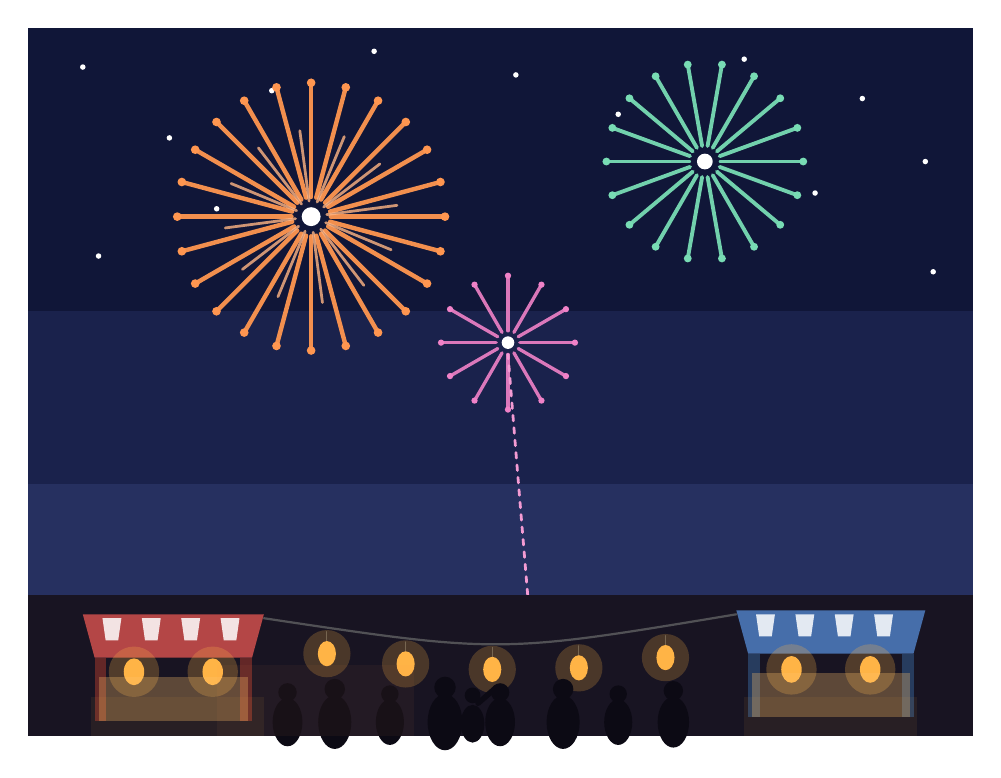
\begin{tikzpicture}[line cap=round,line join=round]
  \definecolor{sky1}{RGB}{16,22,56}
  \definecolor{sky2}{RGB}{26,34,76}
  \definecolor{sky3}{RGB}{38,48,96}
  \definecolor{ground}{RGB}{24,20,34}
  \definecolor{fw1}{RGB}{255,150,80}
  \definecolor{fw2}{RGB}{120,220,180}
  \definecolor{fw3}{RGB}{240,130,200}
  \definecolor{lantern}{RGB}{255,180,70}
  \definecolor{stall1}{RGB}{180,70,70}
  \definecolor{stall2}{RGB}{70,110,170}
  \definecolor{silcol}{RGB}{12,10,20}

  % ---- night sky gradient (banded) ----
  \fill[sky1] (0,5.4) rectangle (12,9);
  \fill[sky2] (0,3.2) rectangle (12,5.4);
  \fill[sky3] (0,1.8) rectangle (12,3.2);

  % stars
  \foreach \p in {(0.7,8.5),(1.8,7.6),(3.1,8.2),(4.4,8.7),(6.2,8.4),
                  (7.5,7.9),(9.1,8.6),(10.6,8.1),(11.4,7.3),(2.4,6.7),
                  (10.0,6.9),(0.9,6.1),(11.5,5.9)} {
    \fill[white] \p circle (0.035);
  }

  % ---- firework 1 (large, orange, center-left) ----
  \begin{scope}[shift={(3.6,6.6)}]
    \foreach \a in {0,15,...,345} {
      \draw[fw1,line width=1.6pt,opacity=0.95] (\a:0.25) -- (\a:1.7);
      \fill[fw1] (\a:1.7) circle (0.055);
    }
    \foreach \a in {7.5,37.5,...,337.5} {
      \draw[fw1!70!white,line width=1pt,opacity=0.8] (\a:0.2) -- (\a:1.1);
    }
    \fill[white] (0,0) circle (0.12);
  \end{scope}

  % ---- firework 2 (green, right, medium) ----
  \begin{scope}[shift={(8.6,7.3)}]
    \foreach \a in {0,20,...,340} {
      \draw[fw2,line width=1.4pt,opacity=0.95] (\a:0.2) -- (\a:1.25);
      \fill[fw2] (\a:1.25) circle (0.05);
    }
    \fill[white] (0,0) circle (0.1);
  \end{scope}

  % ---- firework 3 (pink, lower-middle, small rising burst) ----
  \begin{scope}[shift={(6.1,5.0)}]
    \foreach \a in {0,30,...,330} {
      \draw[fw3,line width=1.2pt,opacity=0.9] (\a:0.15) -- (\a:0.85);
      \fill[fw3] (\a:0.85) circle (0.04);
    }
    \fill[white] (0,0) circle (0.08);
  \end{scope}
  % rising trail of firework 3
  \draw[fw3!80!white,line width=1pt,dash pattern=on 2pt off 2.5pt]
    (6.35,1.8) .. controls (6.25,3.0) .. (6.1,4.85);

  % ---- ground ----
  \fill[ground] (0,0) rectangle (12,1.8);

  % ---- stalls with lanterns ----
  % stall A (left)
  \fill[stall1] (0.7,1.55) -- (3.0,1.55) -- (2.85,1.0) -- (0.85,1.0) -- cycle; % awning
  \foreach \x in {0.95,1.45,...,2.85} { \fill[white,opacity=0.85] (\x,1.5) -- (\x+0.24,1.5) -- (\x+0.2,1.22) -- (\x+0.04,1.22) -- cycle; }
  \fill[stall1!55!black] (0.85,0.2) rectangle (1.0,1.0);
  \fill[stall1!55!black] (2.7,0.2) rectangle (2.85,1.0);
  \fill[lantern] (1.35,0.82) ellipse (0.13 and 0.17);
  \fill[lantern] (2.35,0.82) ellipse (0.13 and 0.17);
  \fill[lantern,opacity=0.25] (1.35,0.82) circle (0.32);
  \fill[lantern,opacity=0.25] (2.35,0.82) circle (0.32);
  % counter glow
  \fill[lantern!80!white,opacity=0.3] (0.9,0.2) rectangle (2.8,0.75);

  % stall B (right)
  \fill[stall2] (9.0,1.6) -- (11.4,1.6) -- (11.25,1.05) -- (9.15,1.05) -- cycle;
  \foreach \x in {9.25,9.75,...,11.05} { \fill[white,opacity=0.85] (\x,1.55) -- (\x+0.24,1.55) -- (\x+0.2,1.27) -- (\x+0.04,1.27) -- cycle; }
  \fill[stall2!55!black] (9.15,0.25) rectangle (9.3,1.05);
  \fill[stall2!55!black] (11.1,0.25) rectangle (11.25,1.05);
  \fill[lantern] (9.7,0.85) ellipse (0.13 and 0.17);
  \fill[lantern] (10.7,0.85) ellipse (0.13 and 0.17);
  \fill[lantern,opacity=0.25] (9.7,0.85) circle (0.32);
  \fill[lantern,opacity=0.25] (10.7,0.85) circle (0.32);
  \fill[lantern!80!white,opacity=0.3] (9.2,0.25) rectangle (11.2,0.8);

  % lantern string between stalls
  \draw[silcol!40!gray,thick] (3.0,1.5) .. controls (6.0,1.05) .. (9.0,1.55);
  \foreach \x/\y in {3.8/1.33,4.8/1.2,5.9/1.13,7.0/1.15,8.1/1.28} {
    \draw[silcol!40!gray] (\x,\y) -- (\x,\y-0.12);
    \fill[lantern] (\x,\y-0.28) ellipse (0.115 and 0.16);
    \fill[lantern,opacity=0.22] (\x,\y-0.28) circle (0.3);
  }

  % ---- crowd silhouettes ----
  \foreach \x/\s in {3.3/0.9,3.9/1.0,4.6/0.85,5.3/1.05,6.0/0.9,6.8/1.0,7.5/0.85,8.2/0.95} {
    \fill[silcol] (\x,0.18) ellipse ({0.21*\s} and {0.34*\s});
    \fill[silcol] (\x,{0.18+0.42*\s}) circle ({0.13*\s});
  }
  % child pointing up at the fireworks
  \fill[silcol] (5.65,0.16) ellipse (0.15 and 0.24);
  \fill[silcol] (5.65,0.52) circle (0.1);
  \draw[silcol,line width=2pt] (5.72,0.42) -- (5.95,0.62);

  % faint reflection of lantern light on the ground
  \fill[lantern,opacity=0.07] (0.8,0.0) rectangle (3.0,0.5);
  \fill[lantern,opacity=0.07] (9.1,0.0) rectangle (11.3,0.5);
  \fill[fw1,opacity=0.05] (2.4,0.0) rectangle (4.9,0.9);
\end{tikzpicture}
\end{document}
